\chapter{Developed Tools}

This chapter contains an overview of why supplementary tools were deemed necessary for an already working reduction process (\S~\ref{sec:polsalt_limits}), which aspects of the reduction process have been altered, replaced, or added (\S~\ref{sec:mod_tools}, \ref{sec:add_tools}), and finally what an updated reduction process consists of using a combination of all software (\S~\ref{sec:red_proc}).


\section{Limitations of POLSALT and the Need for a Supplementary Tool} \label{sec:polsalt_limits} % Rename

% \todo{
%   \begin{itemize}
%     \item Mention difficulty with PG0300?
%     \item Mention GUI difficulties?
%   \end{itemize}
% }

% Why
The creation of supplementary tools for \textsc{polsalt} spectropolarimetric reductions stem from, primarily, the limitations of the wavelength calibration process and a need for a way to compare wavelength solutions across matching $O$ and $E$ polarization beams. Due to the time-consuming process of recalibrating the wavelength solutions it is not feasible to perform the wavelength calibrations time and time again for any amount of reductions larger than a handful of observations.
\prgph

% How
One solution is to use a well established tool to perform the wavelength calibration, one which allows for rapid recalibrations as well as provides a familiar interface with which the user can analyze their wavelength solutions. \textsc{iraf} provides this familiar environment and reliability, even considering it's age and \hyperlink{limited community development}{https://github.com/iraf-community/iraf}. Unfortunately, \textsc{iraf} is unable to parse the file structure implemented by \textsc{polsalt} as is and formatting of the data structures are necessary for integration purposes. This restructuring works both ways as once the \textsc{iraf} reductions are complete the format must be reformatted to match that of the \textsc{polsalt} output such that the reduction process may carry on in \textsc{polsalt}.
\prgph

\todo{The main takeaway should be the need for a way to do the wavelength calibration with more control as well as the need to check the O/E beam wavelength calibrations against one another (since very accurate wavelength calibration necessary for stokes parameter calculations). Feels like something is missing.?}


\section{Wavelength calibrations using the Supplementary Pipeline and IRAF} \label{sec:mod_tools}

The supplementary tools offer an alternate procedure for wavelength calibrations for the \textsc{polsalt} pipeline. This procedure can be broken into three unique steps: the parsing of \textsc{polsalt} data into an \textsc{iraf} friendly format, from here on referred to as splitting; the wavelength calibration performed in \textsc{iraf}; and the reformatting of the data with its wavelength calibration back into the format expected by \textsc{polsalt}, from here on referred to as joining.

\begin{figure}[t]
    \centering
    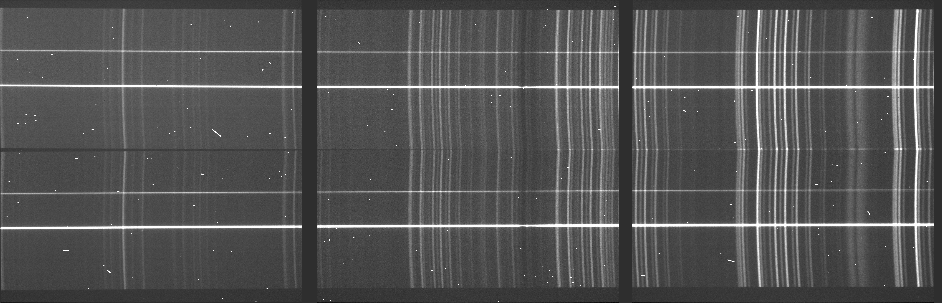
\includegraphics[width = 1.0\textwidth]{figures/3_pre_wav_cal.pdf}
    \caption{The science extension of a typical \textsc{polsalt} \gls{FITS} file after basic \gls{CCD} reductions have been completed.}
    \label{fig:polsalt_pre_wav_cal}
\end{figure}


\subsection{Splitting the POLSALT pre-calibration files}

The main struggle of formatting the files for \textsc{iraf} is that \textsc{iraf} does not handle the chosen \textsc{polsalt} \gls{FITS} file structures well, before or after the \textsc{polsalt} wavelength calibration. A typical \gls{FITS} file created by the \textsc{polsalt} basic \gls{CCD} reductions process has a primary header along with the various image extensions, all of which include both of the polarimetry beams. In an attempt to simplify the \textsc{iraf} reduction procedure it was decided to split the polarization beams into their own files, as the parameters of \textsc{iraf} tasks generally handle lists of files better than lists of cropping regions, and generally allowed for easier calibrations further down the \textsc{iraf} wavelength calibration process.
\prgph

The only steps added to splitting when preparing the \textsc{polsalt} data for \textsc{iraf} was the addition of the ability to crop and the creation of lists for easy automation when performing the wavelength calibrations. The cropping was decided on as \textsc{iraf} does not handle the empty rows and rows with overlapping traces well, specifically when it comes to the \textit{reidentify} task. Otherwise, whenever a design decision had to be made it was decided to stay as true to the \textsc{polsalt} pipeline decision as possible while still allowing \textsc{iraf} to handle the data.
\prgph

The \textsc{polsalt} files with basic \gls{CCD} reductions applied, namely files created by \textsc{polsalt} with a prefix of `mxgbp' (\S~\ref{subsec:polsalt}), are used as the starting point for the supplementary tool's splitting method. Running the split method finds all the \gls{FITS} files for wavelength calibration within the working directory, creates two empty \gls{HDU} structures for each sub-extension of the \gls{FITS} file, and appends all science and header data necessary for wavelength calibration to the relevant \gls{HDU} structure.

Many decisions are made when splitting the data, and it was decided to keep as true to the \textsc{polsalt} pipeline defaults as possible. Presets such as the row along which the data is split, and the amount of cropping applied to the data before appending, are defined but are freely controlled by the user. As this step creates multiple files, it was decided to keep the files for wavelength calibration as light as possible, with only the necessary science extension being copied over.

Fortunately, the \textsc{polsalt} \gls{FITS} files up to and including the basic \gls{CCD} reductions still has a conventional file structure with the only oddity being that the

\todo{Include O/E beam frame example}
\prgph

\todo{Mention steps before and how they return (especially) the file structure.
    All processes run in pipeline split with description of each and purpose. Focus on \textbf{why}.
    Header changes
}

\todo{Parsing polsalt mxgbp frame into something useable by IRAF and making sure the header reflects the changes}


\subsection{IRAF wavelength calibration}\label{subsec:IRAF_wav_cal}

\todo{All wavelength calibration steps - Again, focus on \textbf{why} instead of how
    \begin{itemize}
        \item Identify
        \item Reidentify
        \item Fitcoords
    \end{itemize}
}

\todo{(Optional) Transform (mention good for sanity checks which is not possible using the pure polsalt implementation)}


\subsection{Joining the wavelength calibrated files}

\todo{Return file structuring.}
There are means of accessing inner extensions via indexing within \textsc{iraf}, but this is unreliable for the various \textsc{iraf} tasks. As such, the extension structure needs to be handled such that \textsc{iraf} receives a flattened extension structure with proper extension headers.
\prgph

\todo{All processes run in pipeline join.
    Focus on \textbf{why}. Parsing \textsc{iraf} frames to be used by POLSALT and making sure the header and extensions reflect the changes}

\begin{figure}[t]
    \centering
    \includegraphics[width = 1.0\textwidth]{figures/3_post_wav_cal.pdf}
    \caption{The science extension of a \gls{FITS} file ready to be handed back to the \textsc{polsalt} pipeline.}
    \label{fig:polsalt_pre_wav_cal}
\end{figure}


\section{Additional Tools}\label{sec:add_tools}


\subsection{Cross correlation}

\todo{Why a cross correlation necessary and how it works}


\subsection{Skyline comparisons}

\todo{Again, why a skyline comparison necessary and how it works. Also, how the frame is transformed (\textsc{iraf} bypassed) and that the flux is not conserved so only for checking and not for science use.}


\section{General Reduction Procedure}\label{sec:red_proc}

\todo{General reduction procedure from raw data to finalized results
    \begin{itemize}
        \item This includes \textsc{polsalt} pre-reductions, splitting, \textsc{iraf} wavelength calibrations, checking, joining, and \textsc{polsalt} finalization. (Include Relative flux calibrations for `shape correcting' spectrum??)
    \end{itemize}
}